\documentclass{article}

\usepackage{booktabs} % for toprule, midrule, bottomrule in tables
\usepackage{authblk} % for multiple authors and affiliations
\usepackage[sort&compress,comma,authoryear]{natbib} % for citations
\usepackage{graphicx} % to inlcude graphics with \includegraphics

%packages added by author
\usepackage{hyperref} % to add url hyperlinks in text
\usepackage{multirow} % to combine columns and rows in tables

\author[1,2]{Max Kemman}

\affil[1]{University of Luxembourg, Centre for Contemporary and Digital History}
\affil[2]{Dialogic}

\date{}

\title{Boundary practices of digital humanities collaborations}

\begin{document}

\maketitle

\section*{Abstract}
%intro
One of the defining characteristics of digital humanities is the emphasis on interdisciplinary collaboration. 
To coordinate across disciplinary boundaries, the development of common ground is necessary to negotiate goals and practices.
Yet how such common ground can be established, and whether adoption of interdisciplinary practices and vocabularies leads participants to drift apart from their disciplinary culture, is underexplored.
In this paper I investigate the boundary practices of digital humanities, referring to the interactions of scholars with cross-disciplinary collaborators and disciplinary peers, and how these are configured by disciplinary diversity and physical distance within collaborations.
%question
%method
%With an online survey I have collected 173 responses from digital humanities collaborations.
%results
With an online questionnaire, which received 173 responses,
I find that the disciplinary diversity of digital humanities collaborations is often small, with participants and leadership coming mostly from the humanities. The physical distance is often large, increasingly relying on email.
I do not find that these dimensions affect the respondents' frequency of communication with collaborators or peers.
%conclusion
I conclude that physical distance and disciplinary diversity cannot be confirmed to affect the frequency of boundary interactions of digital humanities.
I furthermore conclude that digital humanities collaborations are biased towards the humanities, rather than a balancing of the digital and the humanities.
This paper thereby provides empirical grounding for discussions of digital humanities as a meeting between the computational domains and the humanities.
%However, the results of the survey present avenues for further exploration necessary to better understand the collaborative practices of digital humanities scholars.

\textbf{Keywords:} collaboration, common ground, communities of practice, survey, boundary practices, interdisciplinarity

 
\section{Introduction}
One of the defining characteristics of digital humanities is the emphasis on interdisciplinary collaboration \citep{Klein2014b,spiro2012}. The different facets of digital humanities research, such as computer technology, data management, and humanistic inquiry, call for experts with different backgrounds to collaborate.
While it is possible for individuals to develop interdisciplinary expertise, collaborations between disciplinary experts may be more effective at providing access to the full range of expertise and practices of disciplines \citep{stokols2006, wilson1996, Siemens2011}.
Diversity of backgrounds in collaborations has consequently been argued to be a prerequisite for the generation of new knowledge in the digital humanities \citep{edmond2016}. 
Yet how collaborations are conducted in the digital humanities is regularly hidden from view and therefore poorly understood \citep{griffin2018}.

The most common conception of digital humanities collaborations assumes they consist of a digital and a humanities side, a collaboration between computational experts and humanities scholars \citep{edmond2005}. 
Digital humanities is then a `meeting place' of these two sides \citep{svensson2011}.
\citet{mccarty2012a} argued this meeting should constitute a `level ground' of mutual collaboration, truly working together rather than computational experts working in service of humanities scholars.
In order to work towards this, it has been argued that collaborators should develop a common ground of shared practices and vocabularies to coordinate goals and practices within the collaboration \citep{Siemens2009,siemens2012human}.
As a result, scholars may learn to translate their humanistic research questions into computational terms \citep{mccarty2012a}.
To illustrate, through continued interactions with computational experts a historian might start to think of their research as testing hypotheses against a historical dataset with the use of algorithms. This will make it easier for this historian to discuss his or her research with computational experts, but might make it more difficult to discuss with other historians not part of a digital humanities collaboration.

Yet how such common ground can be established between different disciplinary discourses, and whether this leads to a drifting apart from one's original disciplinary background are open questions.
Therefore, studying the practices and consequences of collaborations that develop common ground is necessary to better understand the digital humanities as a collaborative practice in itself, and embedded within the humanities at large.

%introduce PhD research

%NEW
A common approach to this question is on a \textit{micro} scale, by interviewing or observing practices of collaboration as they are performed and experienced by individuals or small groups.
Yet whether these individual cases are typical or atypical of the digital humanities more broadly requires contextualisation on the \textit{meso} scale, by quantitatively collecting dimensions of collaborations in a multitude of groups or institutions (see \citealp{edwards2002} for a discussion of the micro and meso scales).
% In my PhD research, collaborations in digital history, as a sub-field of digital humanities, are investigated through a mixed-methods approach \citep{kemman2019}.
% Through a triangulation of methods and perspectives, I have collected observations of collaborative practices on different scales.
% On a \textit{macro} scale, digital history is analysed through a literature review as constituting of large national or global systems or communities.
% On a \textit{meso} scale, digital history is analysed through a questionnaire and observations of institutional politics as constituting of a multitude of institutions or groups.
% Finally, on a \textit{micro} scale, digital history is analysed through interviews and observations of practices as performed and experienced by individuals or small groups (see \citealp{edwards2002} for a discussion of the micro/meso/macro scales).
This paper then concerns the meso scale, by quantitatively exploring the composition of collaborations, and how they configure interactions with cross-disciplinary collaborators and disciplinary peers.
This exploration is based on the findings of the online questionnaire described in Section \ref{sec:method}.
% For the survey, digital humanities more broadly was targeted in order to allow wider distribution and increased responses.
% This paper then serves to contextualise micro analyses of collaborations, in comparing cases as typical or unusual of the organisation of digital humanities.

This paper builds upon the theory of \textit{communities of practice}, %\citep{wenger1998}.
%NEW
defined as the binding together of individuals through a sharing of practices, as experienced in mutual engagement, a joint enterprise, and a shared repertoire of resources \citep[p. 73]{wenger1998}.
In this paper I focus on mutual engagement, the meeting between collaborators, as configured
%The establishment of communities of practice are configured 
through two underlying dimensions that I will elaborate below:
%Two interrelated dimensions that underlie the definition and establishment of communities of practice are of particular interest: 
the shared history of learning %p103
and the geography of practice \citep{wenger1998}. %p130
Using these two dimensions I explore how they lead to different boundary practices between communities of practice, i.e., the interactions between members of different communities.
The communities of interest in this paper then are the humanities, the computational domains, and collaborations as communities consisting of participants from the humanistic and computational communities.

The next section elaborates the two dimensions, after which the questionnaire is introduced and results are discussed.
The paper concludes with lessons learned from the questionnaire and an exploration of research questions that will further our understanding of how digital humanities collaborations work in practice.

\subsection{Dimensions of communities of practice}
The %definition and 
establishment of communities of practice can be described as configured through two underlying dimensions:
the shared history of learning and the geography of practice. 

The first dimension, \textit{shared history of learning}, constitutes the joint adoption of practices and vocabularies through participation and reification of meanings. 
As a shared history of learning how to conduct humanities scholarship, and reification through educating students to be future scholars, the humanities can be thought of as a community of practice.
The same can be said about the computational domains.
These communities of practice demarcate what type of problems are of interest, what types of approaches are suitable, and how research should be communicated, thereby defining the boundaries of disciplinary communities \citep{Becher2001, Gieryn1983}.
The collaboration between the computational domains and the humanities can therefore be seen as a meeting of different histories of learning.
The meeting of shared histories of learning is therefore considered to be the \textit{disciplinary diversity} of a collaboration, and is studied by measuring the extent to which collaborations consist of humanities scholars and computational experts.

The development of common ground can be described as the creation of a new shared history of learning. 
Over time, a common ground might develop into a shared history of learning of a new community of practice that is the union of the digital and the humanities. In this context, several authors have suggested that the digital humanities can indeed be thought of as a community of practice \citep{siemens2013,siemens2016}.

The second dimension, \textit{geography of practice}, refers to the physical locations of collaborators and how that configures interactions. 
The geography of practice stands in a bidirectional relationship with the first dimension, as it influences the likelihood of shaping a shared history of learning.
The most significant aspect is the \textit{physical distance} between collaborators. 
First, distance affects communication. When collaborators are closer together, communication has higher quality, is more frequent, and more often face-to-face \citep{Kiesler2002,Kraut1988}. 
Second, distance affects awareness of collaborators, following the ``out of sight is out of mind'' adage \citep{Olson2002}.
Finally, distance affects the formation of group identity, leading to collaborators speaking in terms of ``us'' and ``them'' \citep{Armstrong2002}.
While disciplinary diversity by itself necessitates coordination to align collaborators, these disciplinary differences have not been found to increase \textit{problems} of coordination, in contrast with physical distance \citep{Cummings2005,Walsh2007}.
Problems of coordination have been found with respect to differences in language and cultural habits, different access to technology, and conflicting requirements from funders \citep{siemens2013}.

This is not to say that physical distance is only a negative aspect, nor does physical proximity guarantee a better collaboration.
Extending physical distance in a collaboration means one can work with the most fitting collaborators, rather than being dependent on who is available nearby \citep{siemens2013}. 
Previous research found that for collaborations within a university, more collaborators correlated with increased negative collaborative experiences. Yet for collaborations between universities this correlation was not found \citep{tsai2016}.
Moreover, physical distance in collaborations can be a strategy for the dissemination of knowledge beyond one's own local network \citep{poole2013}.

Furthermore, `virtual teams' that collaborate mainly through communication technologies such as email or teleconferencing have proven successful, although the formation of mutual trust remains an issue \citep{purvanova2014}.
Face-to-face communication was found to be stronger related to team performance than virtual communication \citep{marlow2018}.
Yet \citeauthor{marlow2018} point to the advantage of what they term `hybrid teams', where complex problems are coordinated face-to-face, while clearer tasks may be coordinated via communication technologies such as email.
Establishing trust and coordinating ill-defined problems, which are common in the digital humanities, therefore benefits from face-to-face meetings throughout a collaboration \citep{siemens2013}.

Physical distance is thus strongly interrelated with communication, a necessary aspect of negotiating common ground. 
This brings me to the next aspect of my study.

\subsection{Boundary practices}\label{sec:boundary-practices}
As a meeting place of different disciplinary communities, digital humanities collaborations can be characterised as \textit{boundary practices}.
Within a collaboration, the development of common ground requires participants to look beyond their own disciplinary identity and engage with collaborators from different backgrounds \citep{Siemens2011a}. 
Participants must be willing to learn about the practices and vocabularies employed by collaborators and integrate them into their own practices for mutual coordination.
As such, interdisciplinary collaborations can be described as practices of crossing one's own disciplinary boundaries.
Collaborations therefore potentially constitute what I term \textit{interdisciplinary boundary crossing}.

Yet a question is how this configures the relationship with a participant's disciplinary community.
It is likely that participants drift away from their disciplinary culture and into a new shared history of learning following the adoption of new vocabularies and practices \citep[p. 103]{wenger1998}.
If scholars wish to discuss their research with disciplinary peers not part of the collaboration, they now find themselves confronted with a boundary of different practices and vocabularies that they did not experience before.
As such, collaborations potentially constitute what I term \textit{intradisciplinary boundary construction}.
For a simplified overview of the boundary practices between the communities of practice see Figure \ref{fig:collabmodel}.

\begin{figure}
\begin{center} 
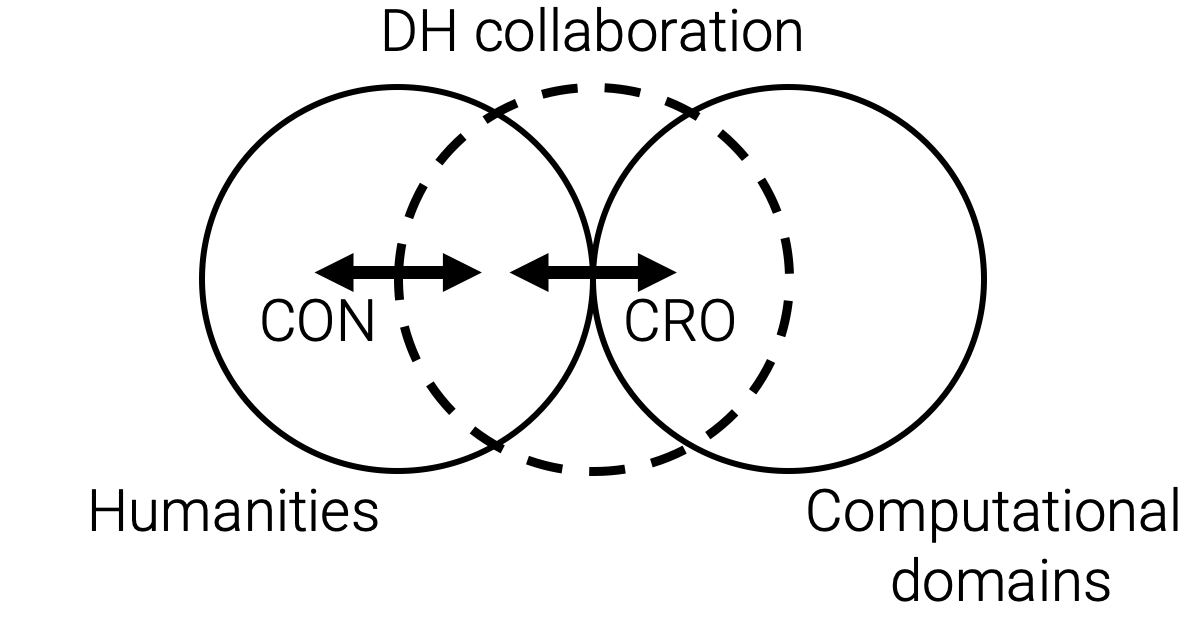
\includegraphics[width=0.7\linewidth]{collabmodelv2.png}  
\caption{Model of a digital humanities collaboration, including intradisciplinary boundary construction (CON) and interdisciplinary boundary crossing (CRO).\label{fig:collabmodel}}  
\end{center}  
\end{figure}

The interactions between the communities of practice that form part of a digital humanities collaboration can therefore be characterised as a duality of interdisciplinary boundary crossing and intradisciplinary boundary construction. 
In the rest of the paper these practices are referred to simply as boundary crossing and boundary construction.
%NEW
This paper explores the boundary practices, disciplinary diversity, and physical distance of digital humanities collaborations. 
Concretely, the research question is the following:
\textit{how do disciplinary diversity and physical distance affect boundary practices of digital humanities collaborations?}


As increased disciplinary diversity is expected to lead to more opportunities for cross-disciplinary interactions within a collaboration, the hypothesis underlying disciplinary diversity is that a small disciplinary diversity, e.g., a collaboration consisting only of historians, will result in less boundary crossing and less boundary construction. 
In contrast, a large disciplinary diversity, i.e., a collaboration consisting of an equal amount of humanities scholars and computational experts,  will result in increased boundary crossing, as well as increased boundary construction.
Furthermore, increased physical distance is expected to make interactions and coordination between cross-disciplinary collaborators more difficult.
In cases of a large physical distance between cross-disciplinary collaborators, it is moreover to be expected that participants will have a small physical distance to their disciplinary peers, since in these cases they are likely to be situated in their disciplinary departments or institutes.
Similarly, a small physical distance to collaborators might mean a large physical distance to disciplinary peers.
The hypothesis underlying physical distance is therefore that a small physical distance, e.g., humanities scholars sharing an office with computational experts, facilitates boundary crossing and boundary construction.
In contrast, a large physical distance is expected to reduce both boundary crossing and boundary construction.

In order to approach the research question and test these hypotheses, 
%NEW
it is necessary to acquire systematic and comparable figures related to these dimensions of digital humanities collaborations.
As such, in this paper I will provide a quantitative outlook on a meso scale.
In the next section I therefore introduce an online questionnaire on collaborative practices in the digital humanities.

\section{Method}
\label{sec:method}

\subsection{Online questionnaire}
The questionnaire was distributed in the period of November 2017 to April 2018 via social media and email. 
The distribution on social media included tweets with hashtags of conferences that occurred during the period that the questionnaire was open. The questionnaire was furthermore distributed in blog posts and through mailing lists. 
Finally, 128 collaborations were emailed based on their affiliation to CenterNet\footnote{CenterNet is an international network of digital humanities centres \citep{walter2012}. I scraped the CenterNet list on 20 November 2017. For a version of the list archived in November 2017 see \url{https://web.archive.org/web/20171029201211/http://dhcenternet.org/centers}} or my awareness of them.
%Finally, I made a list of digital humanities collaborations based on the affiliates of CenterNet and collaborations I was aware of. 
%Based on this list, 128 collaborations were contacted via email.
%I looked up websites and contact persons on this list to request participation in the survey, contacting 128 collaborations in total. 
Invitations for participation were written in English, Dutch, French, German, Spanish, Portuguese, and Italian; the questionnaire itself was in English.

The questionnaire was hosted on a Qualtrics account of the University of Luxembourg.
Respondents were not asked for personally identifiable information in order to preserve anonymity,
%The survey was made anonymous, 
although it did include a question for the name of the collaboration for which a participant was filling out the questionnaire. The main reason this question was included is that many scholars active in digital humanities do not participate in just one collaboration.
In trial runs I noticed participants became confused about which collaboration they were describing in the questionnaire. For example, one participant that worked at a digital humanities centre on a project switched back-and-forth between answers related to the centre and answers related to the project. 
By asking participants to give the name of the collaboration, be it the centre or the project, this name was included in questions so that they were reminded throughout the questionnaire for which collaboration they were providing information. 
The name of the collaboration was not used any further for analysis.

It is therefore possible that several respondents described the same collaboration.
Some statistics that are related to collaborations specifically, such as physical distance and disciplinary diversity, may therefore contain duplicates. However, the inclusion of duplicates need not entail that results are skewed.
Furthermore, the boundary practices reported by respondents are individual. It is possible that within the same collaborations, different participants performed different boundary practices. 
Insofar as this paper aims to investigate whether specific organisations of collaborations lead to specific boundary practices the inclusion of duplicates therefore does not cause problems for analysis.

The questionnaire did not provide a definition of digital humanities or digital history as a prerequisite of participation since both terms are contested in the literature \citep[see e.g.,][]{Antonijevic2015,Robertson2016,Terras2013}.
Likewise, what constitutes a collaboration or who is part of a collaboration is not trivial to define \citep{Katz1997}. 
Whether a certain interaction between scholars or others is considered a collaboration varies between disciplines and institutes \citep{Burroughs2017}. 
For example, CenterNet lists all affiliates as `centres', yet contains a variety of terms such as `lab', `centre', `initiative', `team', `department', `institute', and `group', without a clear delineation between any of these concepts.
Rather than defining types of collaborations, collaborations are defined to exist in mutual recognition as collaborators \citep[p. 56]{wenger1998}.
The questionnaire therefore did not provide a definition of the types of collaboration that were requested for participation, nor who should be thought of as collaborators. 
The questionnaire was thereby designed as a bottom-up approach to investigate the boundary practices of collaborations, rather than a top-down approach of defining types of collaborations and describing the boundary practices for each. 

\subsection{Main units of analysis}
The questionnaire can be consulted in Appendix A. For a structured overview of variables central to the discussion of the research question see Table \ref{tab:variables}. For all variables, respondents could choose a single answer. The range of options and outcomes are described in the next section. 
In this section I describe how these variables relate to the model of digital humanities collaborations as shown in Figure \ref{fig:collabmodel}.

As described above, \textit{physical distance} concerns the distance between collaborators within the collaboration. In Figure \ref{fig:collabmodel}, this concerns anyone falling within the ``DH collaboration'' circle. \textit{Disciplinary diversity} concerns the number of participants from the ``Humanities'' circle and participants from the ``Computational domains'' circle that fall within the ``DH collaboration'' circle. 

With respect to the boundary practices, \textit{intradisciplinary interactions} follows the arrow marked ``CON'' in Figure \ref{fig:collabmodel}, to measure the interactions between participants of the collaboration and their disciplinary peers outside the collaboration.
%within a disciplinary circle between participants falling within the ``DH collaboration'' circle with those outside. 
\textit{Cross-disciplinary interactions} follows the arrow marked ``CRO'' to measure the interactions within the collaboration circle between participants of different disciplinary circles. 
Finally, \textit{main means of communication} concerns the means of communication between collaborators within the ``DH collaboration'' circle.

None of the variables were interval, as shown in Table \ref{tab:variables}, or normally distributed, see appendix B. Therefore, for all statistical tests non-parametric tests will be used.
 
\begin{table}
\caption{Main variables for discussing the research question. The numbers in the column ``Question'' refer to the numbered questions in Appendix A.}
\label{tab:variables}
\makebox[\linewidth]{
\begin{tabular}{@{}llll@{}}

\toprule
Variable & Question & Type & Response rate (\# / \%) \\ \midrule
Physical distance & 9 & Ordinal & 168 / 97 \\
Disciplinary diversity & 5 & Ordinal (Likert) & 173 / 100 \\
Intradisciplinary interactions & 13 & Ordinal & 170 / 98 \\
Cross-disciplinary interactions & 12 & Ordinal & 168 / 97 \\
Main means of communication & 11 & Categorical & 170 / 98 \\ \bottomrule
\end{tabular}
}
\end{table}


\section{Results} 
The questionnaire received 173 responses.\footnote{The data and SPSS code are available open access via Kemman, M. (2019) Boundary practices of digital humanities collaborations. figshare. Dataset. \url{https://doi.org/10.6084/m9.figshare.7813571}}
The replies were analysed using SPSS.
None of the questions were mandatory, and consequently some questions received fewer than 173 replies. 
As this constitutes a relatively small sample size, the analysis below reports both the frequencies of answers as well as percentages.
Statistical tests are considered significant when \textit{p}\textless0.05, following common practices of statistical analysis, and are reported in footnotes accompanying interpretations of results.

The questionnaire collected responses from all continents except Africa. 
Whether this reflects a lack of African digital humanities collaborations or simply a lack of responses is unclear.
%over the world, except African countries.
To geographically contextualise responses, the questionnaire inquired where collaborators were located, allowing multiple answers. 
121 collaborations (70\%) included European partners. European countries with over ten responses were France (22), Germany (24), Italy (19), Luxembourg (15), the Netherlands (28), Switzerland (10), and the UK (27).
47 collaborations included North American partners (27\%), including Canada (14) and the USA (40).
Finally, 32 collaborations included partners from the rest of the world (18\%), without any country with over eight responses.

\begin{table}
\caption{Descriptive aspects of collaborations, reporting both raw frequencies of answers (\#) and the percentage related to all 173 responses (\%).}\label{table:context}
\makebox[\linewidth]{
\begin{tabular}{@{}lll|lll|lll|lll@{}}
\toprule
Time-frame & \# & \%   & Funding        & \# & \%   & Reason        & \# & \%   & Success   & \# & \%   \\ \midrule
Short-term & 95 & 55 & University     & 77 & 45 & Topic         & 45 & 26 & Yes       & 89 & 52 \\
Semi-long  & 33 & 19 & National       & 84 & 49 & PI            & 33 & 19 & No        & 5  & 3  \\
Long-term  & 44 & 25 & European       & 23 & 13 & Career        & 19 & 11 & Too early & 31 & 18 \\
           &    &      & Government     & 22 & 13 & Collaboration & 14 & 8  & Partially & 12 & 7  \\
           &    &      & Infrastructure & 9  & 5  & Methods       & 13 & 8  & Can't say & 4  & 2  \\
           &    &      & Other          & 43 & 25 & Novelty       & 6  & 3  &           &    &      \\
           &    &      &                &    &      & Other         & 10 & 6  &           &    &    \\
\bottomrule
\end{tabular}
}
\end{table}

To further contextualise the type of collaborations, the questionnaire included questions about the time-frame (single-choice) and the source of funding (multiple choices).
With respect to the time-frame, respondents could choose between short-term (deadline within four years), semi-long term (longer than four years or without a concrete deadline), or long-term (no deadline).
Although four years is already relatively long, especially for computational projects, this captures projects tied to PhD positions and most fixed-term contracts.
The majority of collaborations were short-term, see Table \ref{table:context}.
With respect to funding, 
%it is of interest that 
the split between university funding and funding from a national funding agency was fairly balanced.

The questionnaire furthermore 
%included a question regarding 
inquired about
contractual responsibilities of collaborators, where respondents could choose multiple answers. For the majority of collaborations, participants worked on multiple research projects (129, 75\%). Only 17 respondents (10\%) indicated that participants were contractually tied solely to the one specific collaboration. 

Finally, the questionnaire included open-ended questions about the respondent's individual reason to join, and whether they considered the collaboration a success. Both questions were manually coded for analysis by grouping similar answers under a single category.
The most frequent reason to join a collaboration was interest in its topic, see Table \ref{table:context}.
Two other types of responses are particularly interesting. The second most common response was that the respondent was the PI or founder of a collaboration. This is hardly an explanation why a respondent chose to participate in a collaboration but suggests a different incentive between PIs and others who join the collaboration later on. It appears that PIs do not join a collaboration but establish it, and consequently have no other reasons for joining.
Another response of interest is that several respondents indicated they joined as part of their career, either because this is a collaboration tied to a position they replied to, available funding for research, or as part of their job responsibilities. 
This suggests participation in digital humanities collaborations may in some cases follow top-down decisions rather than intrinsic interests.

With respect to the success of a collaboration, the majority of respondents considered their collaboration a success, see Table \ref{table:context}. Only five respondents answered negatively.
I cannot assume or conclude that this is representative of the success of digital humanities collaborations in general.
It could be a result of self-selection bias for the question, as several respondents did not answer the question. Furthermore, this finding could show self-selection bias for the questionnaire, with scholars in successful collaborations more likely to respond to a questionnaire about their collaboration. The questionnaire did not further request an explanation why a collaboration was deemed successful or not.

Having contextualised the responses as such, the following sections focus on the boundary practices central to this paper, and how they are configured by disciplinary diversity and physical distance.

\subsection{Disciplinary diversity}
With respect to the first dimension, disciplinary diversity, I consider three categories of possible answers as disciplinary backgrounds.
First, \textit{humanities backgrounds}, consisting of the possible answers `history', `other humanities', or `cultural heritage'.\footnote{The separation between history and other humanities is a result of this questionnaire being conducted as part of my PhD research on digital history specifically \citep{kemman2019}.}
Second, \textit{computational backgrounds}, consisting of the possible answers `computer science', `computational linguistics', or `software development'.
Finally, other possible answers were `library' and `other'.
Three questions inquired about disciplinary diversity.

\begin{table}
\centering
\caption{Disciplinary diversity. Frequencies (\#) and percentages of all 173 responses (\%).}
\label{table:discdiversity}
\begin{tabular}{@{}lllll@{}}
\toprule
\multirow{2}{*}{}            & \multicolumn{2}{l}{\textbf{Leadership}} & \multicolumn{2}{l}{\textbf{Participants}} \\
                             & \#          & \%                 & \#           & \%                  \\ \midrule
History                      & 88                 & 51               & 102                 & 59                \\
Other humanities             & 82                 & 47               & 109                 & 63                \\
Cultural heritage            & 22                 & 13               & 50                  & 29                \\
\textbf{Humanities total}    & \textbf{157}       & \textbf{91}      & \textbf{150}        & \textbf{87}       \\ \midrule
Computer science             & 23                 & 13               & 83                  & 48                \\
Computational linguistics    & 18                 & 10               & 43                  & 25                \\
Software development         & 13                 & 8                & 75                  & 43                \\
\textbf{Computational total} & \textbf{40}        & \textbf{23}      & \textbf{127}        & \textbf{73}       \\ \midrule
Library                      & 21                  &       12           & 51                  & 31             \\
Other                        & 35                 & 20                 & 54                  & 31              \\  
\bottomrule
\end{tabular}
\end{table}

The first two questions concerned the disciplinary background of the leadership of the collaboration and of other participants. Respondents could choose multiple answers for both questions.
For an overview of responses see Table \ref{table:discdiversity}.
With respect to the disciplinary diversity of leadership, \textit{collaborations were mostly led by humanities scholars}: 91\% included humanities scholars in leadership, compared to 23\% that included computational experts.
Furthermore, the majority of collaborations were led \textit{exclusively} by scholars with a humanities background (126, 73\%). A much smaller number of collaborations were led exclusively by people with a computational background (9, 5\%). For 31 collaborations (18\%), leadership involved scholars both from the humanities and from a computational background.

With respect to the other participants of collaborations, disciplinary diversity appears more balanced. 
\textit{Most collaborations included participants with a humanities background and participants with a computational background}: 87\% of collaborations included humanities scholars, and 73\% included computational experts.

The third question concerned the ratio of humanities scholars to computational experts on a 5-point Likert scale.
\textit{For the vast majority of collaborations, humanities scholars outnumbered computational experts}. 
For an overview see Figure \ref{fig:piediscdiversity}. Collaborations with only humanities scholars or mostly humanities scholars together comprise three-quarters of all responses. No collaborations included only computational experts.

\begin{figure}  
\begin{center}  
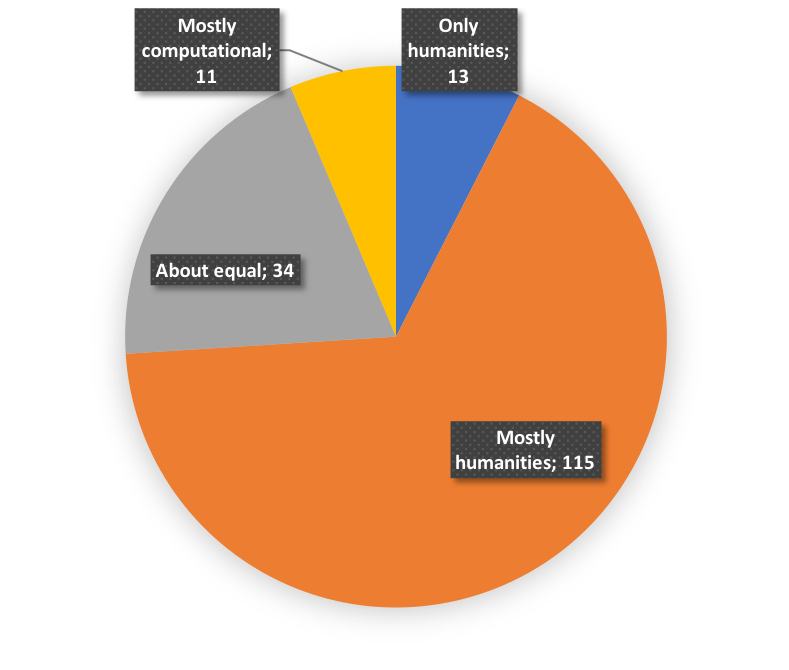
\includegraphics[width=0.6\linewidth]{piediscdiversity.png}  
\caption{Ratio of disciplinary backgrounds.\label{fig:piediscdiversity}}  
\end{center}  
\end{figure}

In summary, \textit{the disciplinary diversity of digital humanities collaborations was often small}: leadership consisted mostly of humanities scholars, and for other participants humanities scholars outnumbered collaborators with a computational background. 

\subsection{Physical distance}
With respect to the second dimension, physical distance, three questions were related to where collaborators conducted their work and how they communicated with one another.

First, respondents were asked where the main participants of the collaboration worked, allowing a single answer.  This concerns the \textit{main} participants of collaborations, since from my own observations collaborations are often officially led by professors who have their own offices, but mainly conducted by researchers in PhD or postdoc positions who might or might not be sharing an office together. It is the interactions of these main participants that are of particular interest for the development of common ground.
The frequencies of responses to this question can be seen in Figure \ref{fig:bardistance}. A total of 34 collaborations (20\%) were conducted on a very short distance in a single space, either a lab or an office. 42 collaborations (24\%) were conducted further apart, but still within a single institute. Finally, 92 collaborations (53\%) were conducted between multiple institutes in national or international contexts. As such, \textit{the majority of collaborations were conducted on a large physical distance}.

\begin{figure}  
\begin{center}  
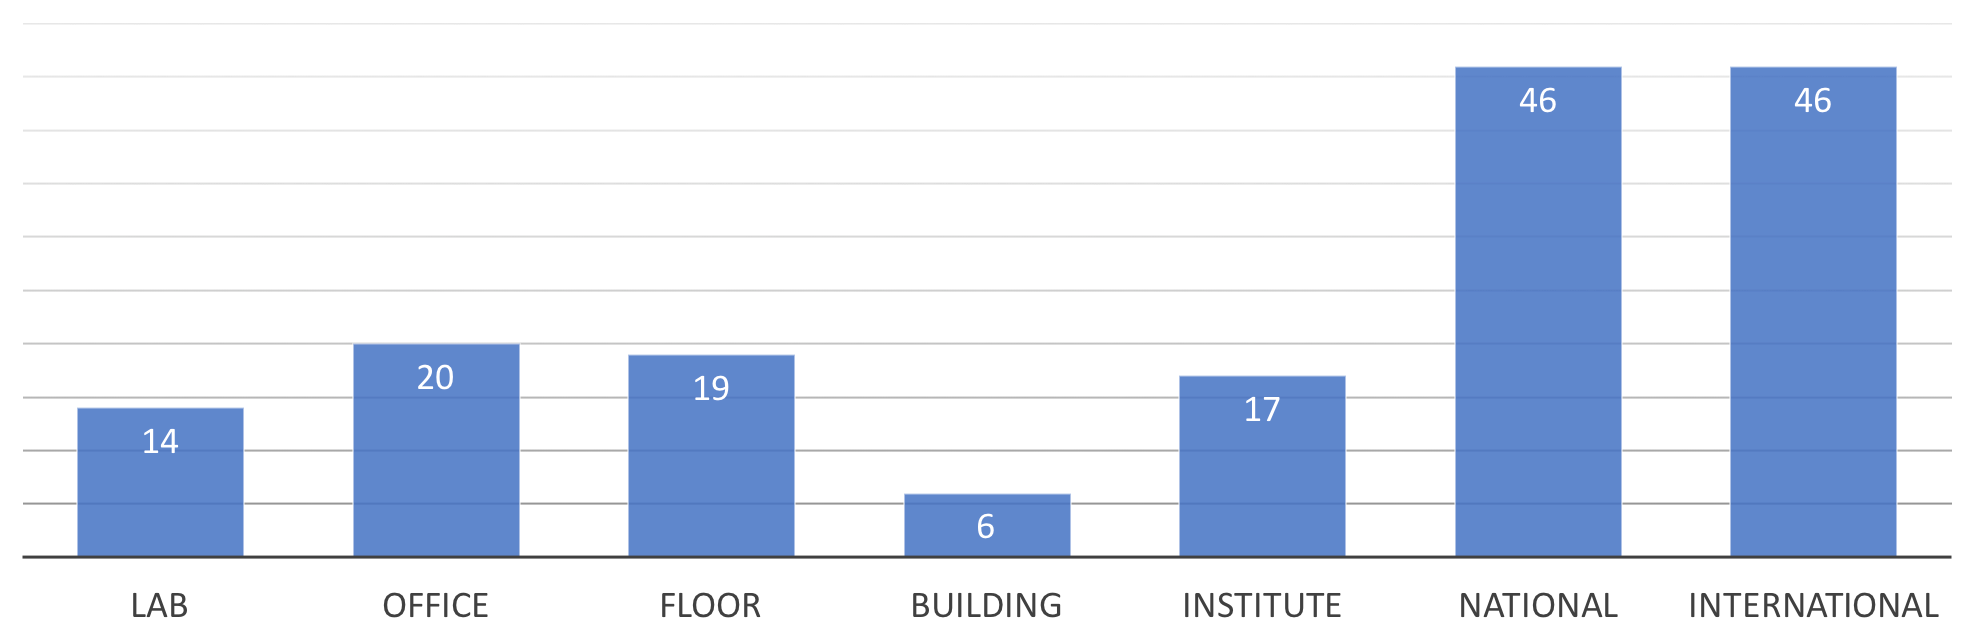
\includegraphics[width=1.0\linewidth]{bardistance.png}  
\caption{Physical distance between main collaborators, showing the frequencies of responses.\label{fig:bardistance}}  
\end{center}  
\end{figure}

A second question concerned the institutional buildings where these spaces were located, allowing multiple answers. The majority of collaborations were located in the humanities building of an institute (112, 65\%). Far fewer collaborations had spaces in the computer science building (29, 17\%) or the library building (32, 18\%). This corresponds to the earlier finding that the majority of collaborations consisted mainly of scholars from the humanities.

The final question inquired about the main means of communication within the collaboration, allowing a single response. 
In Figure \ref{fig:barcomms} it can be seen that physical distance affected communication within a collaboration:\footnote{The category ``offices on multiple floors in a single building'' received only six responses, and all six communicated  face-to-face. This distribution of answers is different from the other categories, which I assume is a result of the small sample size rather than a meaningful consequence of this category of physical distance. This category is therefore excluded from subsequent analyses.} 
\textit{as physical distance increased, the use of face-to-face communication decreased, and the use of email increased},\footnote{I tested the relation between physical distance and communication via email or face-to-face with Kendall's tau correlation, a non-parametric test for ordinal data with small sample sizes \citep[pp. 181-182]{Field2009}. Considering both variables are ordinal, tau-c was used to control for so-called `tied ranks' where multiple respondents chose the same answers. Only cases that mainly communicated via email or face-to-face were selected, and the six responses in the category ``offices on multiple floors in a single building'' were left out (see footnote 4). For the remaining 129 cases larger physical distance was found to be significantly correlated to more email instead of face-to-face communication $\tau$-c=0.445, \textit{p}(two-tailed)\textless0.001, N=129.}
in agreement with the literature.
Within a lab the use of face-to-face over email appears different from a single office, indicating different styles of collaboration in different spaces. 
Moreover, when the collaboration was spread out over multiple buildings in a single institute, the use of email increased to a similar level as for multiple institutes or international collaborations. This seems to indicate that inter-departmental collaborations experience similar thresholds to face-to-face communication as inter-institutional collaborations.

\begin{figure}  
\begin{center}  
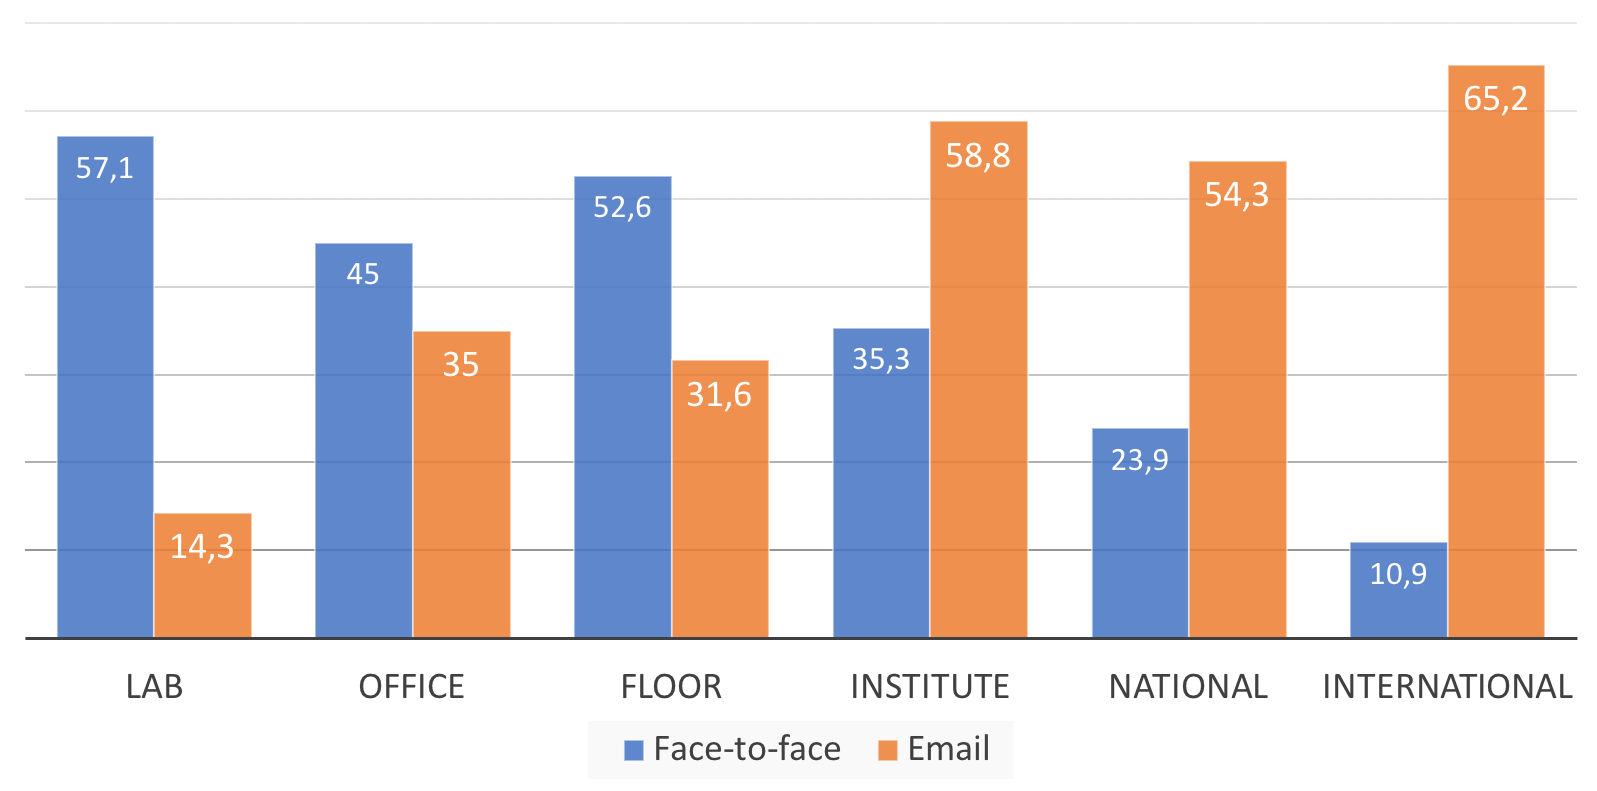
\includegraphics[width=1.0\linewidth]{barcomms.png}  
\caption{Main means of communication within the collaboration per distance, showing the percentage of responses.\label{fig:barcomms}}  
\end{center}  
\end{figure}

In summary, \textit{the physical distance of digital humanities collaborations was often large}: the majority of collaborations were conducted between different institutes, increasingly depending on email rather than face-to-face communication.

\subsection{Boundary practices}
As described above, two forms of boundary practices are central to the current study: interdisciplinary boundary crossing and intradisciplinary boundary construction. 
As a proxy for these boundary practices, the questionnaire inquired about the frequency of research-related communication with cross-disciplinary collaborators and disciplinary peers.
Figure \ref{fig:barboundary} shows the frequency of responses to both questions in comparison.
From this figure it can be seen that both disciplinary and interdisciplinary communication were quite frequent. Two-thirds of respondents spoke at least weekly with interdisciplinary collaborators. Three-quarters of respondents spoke at least weekly with disciplinary peers.
Interaction with disciplinary peers outside the collaboration was significantly more frequent than interdisciplinary communication within the collaboration.\footnote{I tested the difference with a Wilcoxon signed-rank test, a non-parametric test of differences between two sets of answers originating from the same respondents \citep[pp. 552-558]{Field2009}. Respondents communicated significantly less with cross-disciplinary collaborators with \textit{z}=-2.301, \textit{p}(two-tailed)\textless0.05, N=168, \textit{r}=-0.13.}

Tests on the relation between disciplinary diversity or physical distance and boundary practices all returned non-significant results.\footnote{I tested these relations with Fisher's exact test, a test to compare the relationship between non-interval variables with small sample sizes \citep[p. 690]{Field2009}. This concerns four independent statistical tests, none of which showed a statistically significant relation:
1) disciplinary diversity related to interdisciplinary communication, \textit{p}(two-tailed)=0.08, 2) disciplinary diversity related to disciplinary communication, \textit{p}(two-tailed)=0.52 3) physical distance related to interdisciplinary communication, \textit{p}(two-tailed)=0.12 and 4) physical distance related to disciplinary communication, \textit{p}(two-tailed)=0.25.
}
In other words, \textit{I find no signs that disciplinary diversity or physical distance affected the frequency of intradisciplinary or interdisciplinary boundary interactions}.
%\todo{Meaningful to add? disciplinary communication and interdisciplinary communication appear to be correlated in the sense that scholars that communicate more often disciplinary also communicate more often interdisciplinary}

\begin{figure}  
\begin{center}  
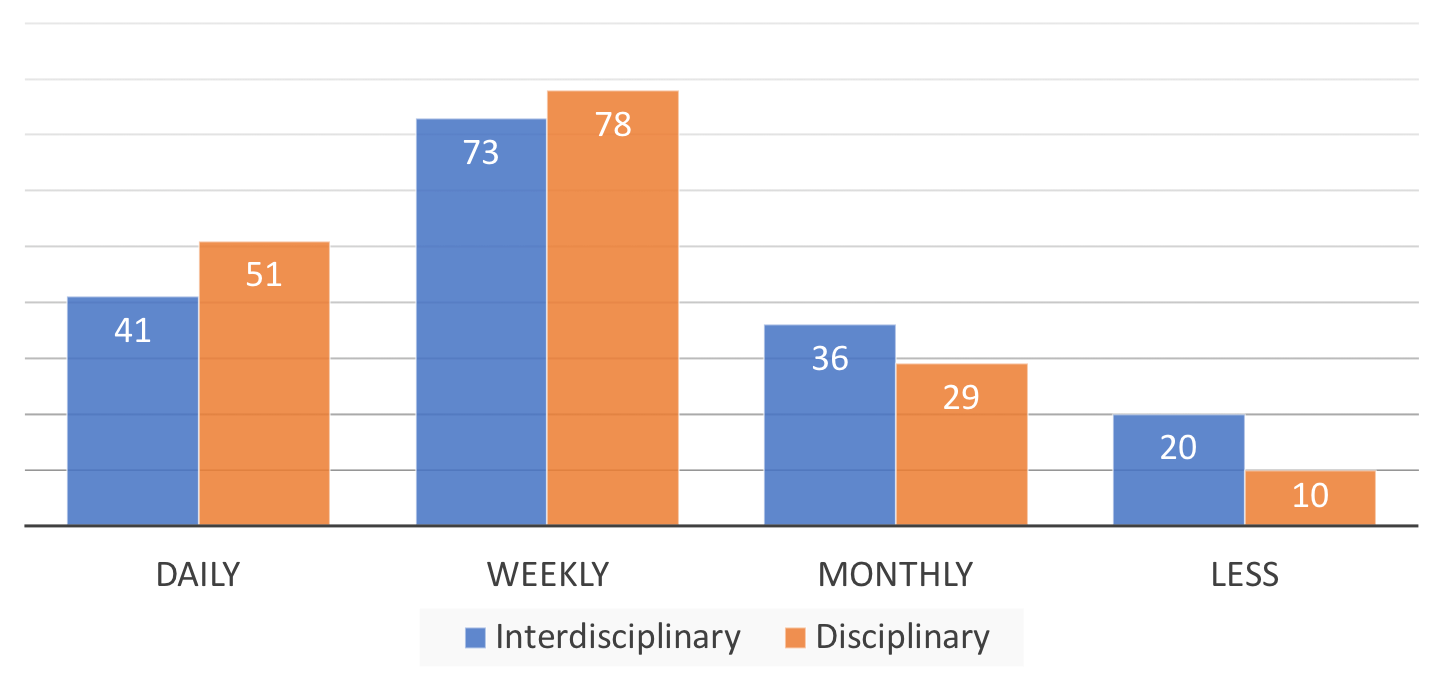
\includegraphics[width=1.0\linewidth]{barboundary.png}  
\caption{Frequencies of interactions with cross-disciplinary collaborators or disciplinary peers, showing the frequency of responses.\label{fig:barboundary}}  
\end{center}  
\end{figure}

\section{Discussion}

In summary, the questionnaire found that the disciplinary diversity of digital humanities collaborations was often small; participants of collaborations were mostly from the humanities, and most collaborations were led by humanities scholars.  
The majority of collaborations were conducted across a large physical distance, which correlated with an increased dependence on distant communication via email rather than face-to-face.

I hypothesised that a small disciplinary diversity and a large physical distance would both lead to a decreased opportunity for interdisciplinary boundary crossing, and decreased intradisciplinary boundary construction.
%Following my hypotheses described earlier in this paper, I expected these findings to result in little interdisciplinary boundary crossing and little boundary construction.
%If this were the case, this would mean that most digital humanities collaborations essentially do not constitute new communities of practice, but participants remain aligned with their disciplinary community of practice. 
However, the analyses did not confirm that disciplinary diversity or physical distance affected the frequency of boundary interactions. The hypotheses therefore cannot be confirmed.
%As such, disciplinary diversity and physical distance do not appear to be conditions for the formation of communities of practice in the sense that one can predict the formation of one from the conditions.
%A collaboration with large disciplinary diversity and a small physical distance is thus no guarantee for the formation of a new shared history of learning. 
%This is intuitive on a small-scale, in the sense that collaborations can fail or fall apart for a number of contingent reasons.
Yet a number of findings give further insights into the boundary practices that may affect the development of common ground in digital humanities collaborations.

First, while physical distance did not affect the \textit{frequency} of interactions, it did affect the \textit{nature} of communication in the collaborations, 
as increased physical distance was related to increased reliance on email.
%increasingly relying on distant communication techniques.
However, previous research found digital communication insufficient for the development of common ground \citep{Siemens2009}.
Especially insofar as collaborations need to establish mutual trust and coordinate ill-defined goals, it has been questioned whether distant communication can facilitate this \citep{sonderegger2009}.
In such situations, goals emerge through continuous negotiations, instead of being established prior to the collaboration \citep{haythornthwaite2006}.
It is therefore that collocation, such as sharing an office, has been found to facilitate the development of common ground most effectively \citep{Olson2002}.

Second, for the majority of collaborations participants worked on multiple projects. This suggests that even if a common ground is established in a collaboration, these shared practices and vocabularies are limited to the collaboration. 
For other collaborations, it is to be expected that participants need to negotiate other common grounds. 
The opportunity for a common ground to develop into a shared history of learning thus appears limited.

Third, the majority of collaborations were embedded in the humanities buildings of institutes. This suggests smaller physical distance to disciplinary peers for participants from the humanities.

Finally, respondents communicated significantly more with disciplinary peers outside the collaboration than cross-disciplinary collaborators.
These last two findings suggest that humanities scholars remained aligned with their humanities background, rather than form a new alignment with computational collaborators. 
It thus appears unlikely that the humanities scholars of digital humanities drift apart from their disciplinary community.
Considering collaborations were furthermore predominantly conducted and led by humanities scholars, my findings agree with \citet{svensson2011} when he characterises ``the digital humanities as a humanities project'' in the title of his paper. 
Digital humanities thus appears less diverse than assumed \citep[c.f.][]{edmond2016}.

\section{Conclusions and future outlook}
In conclusion, let me return to the research question underlying this paper: \textit{how do disciplinary diversity and physical distance affect boundary practices of digital humanities collaborations?}
Answering this question is not straight-forward. 
Disciplinary diversity and physical distance did not affect the frequency of boundary interactions.
I therefore did not find effects of these dimensions on boundary crossing or boundary construction.
Yet physical distance did affect the nature of communication, with increased physical distance related to increased reliance on email.
The questionnaire moreover found that the majority of collaborations were conducted over a large distance with predominant participation from humanities scholars. 
I therefore conclude that digital humanities collaborations are biased towards the humanities, rather than a balancing of the digital and the humanities.
The main contribution of this paper then is to provide empirical grounding for discussions of digital humanities as a meeting between the computational domains and the humanities.
The results of this paper furthermore facilitate the contextualisation of future case studies of digital humanities collaborations, in positioning their organisation as typical or atypical compared to the results of the questionnaire.

%While disciplinary diversity and physical distance did not affect the frequency of boundary practices, they may have ramifications for collaborations that could not fully be explored with an online survey.

The approach described in this paper
thereby provides a quantitative meso perspective on collaborations, yet
presents a number of limitations that affect interpretability. 
A first limitation is that most respondents were likely from the humanities, as a result of my distribution methods. This could have skewed findings insofar as humanities scholars outnumbered other disciplinary backgrounds. For example, collaborations between computational experts and cultural heritage, which may well be considered digital humanities practices, are probably underrepresented. 
Second, by focusing on disciplinary diversity, physical distance and boundary practices the questionnaire managed to investigate collaborations through a quantitative approach. However, this does not provide in-depth insights into the development of common ground, the establishment of boundary practices, or the nature of practices in the digital humanities.
For example, since the majority of respondents indicated that participants worked in multiple collaborations, a much more granular look at how individuals move between collaborations and perform boundary practices is necessary.
Therefore, following the results of this questionnaire, a number of questions for future research require further exploration.

First, considering the apparent predominant participation and leadership from humanities scholars, a question is how this affects possible power relations in interdisciplinary collaborations. 
While \citet{mccarty2012a} argued for a level ground where computational experts work with rather than in service of humanities scholars, it is possible that humanities scholars effectively set the agenda for digital humanities collaborations.
How such power relations affect the development of common ground and the coordination of practices requires deeper observations of the interactions between humanities scholars and computational experts.
For example, a question is whether commonly negotiated vocabularies lie closer to the disciplinary discourses of the humanities, or to that of computational domains.

Second, considering the dependence on communication technology such as email, a question is how this affects the development of common ground.
Since communication technology has been found lacking in previous research, distant collaborations may need to plan for face-to-face meetings at partners' locations in order to develop common ground \citep{siemens2013,sonderegger2009}.
Yet whether such meetings at intervals are sufficient is underexplored.
In the case of communication technology, email has been found to be the best alternative to face-to-face, rather than synchronous distant communication. 
The reason is that email allows collaborators to contemplate and elaborate what they intend to communicate, and also provides a stable backlog that can facilitate common ground \citep{sonderegger2009}. 
More research is therefore needed regarding how communication technologies are used to develop common ground in the digital humanities.

Finally, the relation between the digital humanities and the humanities at large deserves more attention.
A question is whether scholars ultimately remain part of their disciplinary culture, or whether the digital humanities indeed constitute a distinct community of practice \citep{siemens2013, siemens2016}.
In this context, digital humanities has been suggested to constitute a ``dual citizenship'' \citep{Svensson2012}, or a third culture \citep{Hunter2014} between the digital and the humanities.
Yet the results from the questionnaire suggest otherwise. 
Scholars remained in close contact with disciplinary peers. 
%Most scholars were part of multiple collaborations, so that it is possible that different vocabularies become common ground in different collaborations, not extending beyond any single collaboration. 
%NEW ALternative?
Most scholars were part of multiple collaborations, rendering it likely that scholars developed and negotiated different practices in different settings. This raises the question whether vocabularies and practices shared within a single collaboration are able to extend beyond that collaboration into a wider community of practice of digital humanities.

On the meso scale adopted in this paper, the digital humanities therefore appears to maintain the duality of the humanities and the computational sides.
Yet the results suggest that the digital humanities may be more humanities than in-between.
%NEW
While on a micro scale scholars may act in-between, possessing both humanistic and computational skills, these cases appear atypical to the wider context of digital humanities collaborations.
This is not to deny the possibility of digital humanities as a third space, but poses questions about how scholars develop into members of such a third space, how exactly this third space relates to the humanities and the computational domains, and what kind of boundary practices this introduces.

\section*{Acknowledgements}
I would like to thank a number of people for help and feedback that helped improve this paper.
Anita Lucchesi, Benjamin Zenner, Lucas Duane, Stef Scagliola, and Vitus Sproten who translated the invitations to the questionnaire.
Andreas Heinz who provided feedback on the statistical tests.
Christopher Morse who proof-read the article. 
The editors and anonymous reviewers who provided feedback on an earlier version of this paper.
The questionnaire reported in this paper is part of my PhD thesis on trading zones of digital history, supervised by Andreas Fickers, Beno\^it Majerus and Pelle Snickars. I thank them for their feedback on an earlier version of this paper. 

% The reference list will be generated automatically based on the keys 
% you use in your article and their metadata in the bibtex file
\bibliographystyle{humannat}
\bibliography{selected-bib}

\newpage

\section*{Appendix A - Questionnaire}

\begin{enumerate}
    \item What is the name or title of your collaboration? (text input)
    \item Where are people participating in \texttt{Q1-answer} located? (multiple choices)
    \item From what backgrounds does leadership (director, PI, supervisor, or otherwise) come? (multiple options)
    \begin{itemize}
        \item History
        \item Other humanities disciplines
        \item Computational linguistics
        \item Computer science
        \item Cultural heritage
        \item Library
        \item Software development
        \item Other (text input)
    \end{itemize}
    \item From what backgrounds do participants other than leadership come? (multiple choices)
    \begin{itemize}
        \item History
        \item Other humanities disciplines
        \item Computational linguistics
        \item Computer science
        \item Cultural heritage
        \item Library
        \item Software development
        \item Other (text input)
    \end{itemize}
    \item Are participants mostly from a humanities background or mostly from a computational background? (single choice)
    \begin{itemize}
        \item Only from a humanities background
        \item Mostly from a humanities background
        \item About equal
        \item Mostly from a computational background
        \item Only from a computational background
    \end{itemize}
    \item Which of the following statements is true about \texttt{Q1-answer}? (multiple choices)
    \begin{itemize}
        \item Participants are all contractually tied solely to \texttt{Q1-answer}
        \item Participants are all contractually tied to the same organisational unit (not necessarily \texttt{Q1-answer})
        \item Participants are contractually tied to other organisational units than \texttt{Q1-answer}
        \item Participants have a dual position in their contract, \texttt{Q1-answer} and another organisational unit
        \item Participants are contractually tied to different institutions
        \item Participants work only on the \texttt{Q1-answer}
        \item Participants work on multiple research projects
        \item Participants perform user research engaging humanities scholars not part of \texttt{Q1-answer}
    \end{itemize}
    \item What is the time frame of \texttt{Q1-answer}? (single choice)
    \begin{itemize}
        \item Short term (working towards deadline within 4 years)
        \item Semi-long term (no concrete deadline or more than 4 years)
        \item Long term (no deadline)
    \end{itemize}
    \item What is the source of funding? (multiple choices)
    \begin{itemize}
        \item University
        \item National funding agency
        \item European funding agency
        \item Government (other than national funding agency)
        \item Another infrastructure project (e.g. DARIAH, CLARIN)
        \item Other (text input)
    \end{itemize}
    \item What is the physical space where the main participants of \texttt{Q1-answer} work? (single choice)
    \begin{itemize}
        \item Lab space
        \item Single office
        \item Multiple offices on a single floor
        \item Multiple offices on multiple floors in a single building
        \item Offices in multiple buildings of a single institution
        \item Offices in multiple institutions in a single country
        \item Offices in multiple institutions in multiple countries
    \end{itemize}
    \item Where is the space or are spaces located (multiple choices)
    \begin{itemize}
        \item In the library building
        \item In the humanities building
        \item In the computer science building
        \item Other (text input)
    \end{itemize}
    \item How do you mainly communicate with other participants? (single choice)
    \begin{itemize}
        \item Face to face
        \item Video conferencing
        \item Telephone conferencing
        \item Email
        \item Slack
        \item Other communication platform(s) (text input)
    \end{itemize}
    \item How often do you communicate about research-related matters with participants from a different disciplinary background than your own? (single choice)
    \begin{itemize}
        \item Daily
        \item Weekly
        \item Monthly
        \item Every 2-6 months
        \item Annually
        \item Never
    \end{itemize}
    \item How often do you communicate about research-related matters with people from your own disciplinary background, that are not part of \texttt{Q1-answer}?
    \begin{itemize}
        \item Daily
        \item Weekly
        \item Monthly
        \item Every 2-6 months
        \item Annually
        \item Never
    \end{itemize}
    \item Of what organisational unit(s) is the lab a part? (multiple choices)
    \begin{itemize}
        \item Entirely independent
        \item The digital history/digital humanities group
        \item The humanities faculty
        \item The computer department
        \item The library
        \item Other (text input)
    \end{itemize}
    \item Which of the following does the lab provide? (multiple choices)
    \begin{itemize}
        \item Computers
        \item Scanners
        \item Printers
        \item Personnel (such as software developers)
        \item Other (text input)
    \end{itemize}
    item Which of the following statements is true about the lab? (single choice)
    \begin{itemize}
        \item The lab is meant for people contractually tied to the same organisational unit as the lab
        \item The lab is open to anyone from the humanities in the university
        \item The lab is open to anyone from history in the university
        \item The lab is open to anyone in the university
        \item Other (text input)
    \end{itemize}
    \item Please describe in short the goal of \texttt{Q1-answer}? (text input)
    \item What is your individual reason for joining \texttt{Q1-answer}? (text input)
    \item Would you say \texttt{Q1-answer} is successful? (text input)
\end{enumerate}

\newpage

\section*{Appendix B - Kolmogorov-Smirnov tests}
\label{appB}
%\subsection*{}
None of the variables used in this paper were normally distributed, as found through Kolmogorov-Smirnov tests, a test for normal distribution \citep[pp. 144-148]{Field2009}:

\begin{itemize}
\item Disciplinary diversity D(166)=0.38, \textit{p}\textless0.01
\item Physical distance D(166)=0.25, \textit{p}\textless0.01
\item Intradisciplinary interactions D(166)=0.28, \textit{p}\textless0.01
\item Cross-disciplinary interactions D(166)=0.27, \textit{p}\textless0.01
\item Main means of communication D(166)=0.31, \textit{p}\textless0.01
\end{itemize}

\end{document}

\section{References}
\label{sec:references}